\documentclass[areasetadvanced]{scrartcl}

\usepackage[utf8]{inputenc}
\usepackage[T2A]{fontenc}
\usepackage[english,russian]{babel}

\usepackage[footskip=1cm,left=25mm, right=15mm, top=20mm, bottom=20mm]{geometry}
\usepackage{setspace}
\usepackage{amsmath, amssymb}  % Объединено в одну строку
\usepackage{graphicx}
\usepackage{tikz}
\usetikzlibrary{arrows.meta}
\usepackage{float}
\usepackage{dashrule}
\usepackage{fancyhdr} % оформление отчёта
\usepackage{hyperref} % оформление отчёта
\usepackage{parskip}
\usepackage{textcomp, enumitem}
\usepackage{indentfirst}
\usepackage{graphicx}
\usepackage{algorithm}
\usepackage{algpseudocode}
\usepackage{tocloft}
\usepackage{array}  % Для использования команды m{}
\usepackage{geometry}
\usepackage{afterpage}
\usepackage{minted}
\setlength{\parindent}{1.25cm}   % Включает subsubsection в содержание
\usepackage{listings} % Если используете listings

\tikzstyle{block} = [rectangle, rounded corners, minimum width=3cm, minimum height=1cm, text centered, draw=black, fill=lightgray]
\setcounter{tocdepth}{3}
\setcounter{secnumdepth}{3}
\setkomafont{sectioning}{\normalfont\bfseries} % для заголовков разделов и подразделов
\setkomafont{section}{\normalfont\Large\bfseries}
\setkomafont{subsection}{\normalfont\large\bfseries}
\setkomafont{subsubsection}{\normalfont\large\bfseries}
\setkomafont{paragraph}{\normalfont\large\bfseries} % для заголовков параграфов (если они есть)

\lstset{
  language=Java,
  basicstyle=\ttfamily\small,
  keywordstyle=\color{blue}\bfseries,
  stringstyle=\color{red},
  commentstyle=\color{green!70!black},
  numbers=left,
  numberstyle=\tiny,
  stepnumber=1,
  numbersep=10pt,
  showstringspaces=false,
  breaklines=true,
  frame=single
}

\begin{document}
\sloppy
	\thispagestyle{empty}
	\begin{center}
		\large{МИНОБРНАУКИ РОССИИ} \par
		\vspace{0.3cm}
		\normalsize
		{ФЕДЕРАЛЬНОЕ ГОСУДАРСТВЕННОЕ АВТОНОМНОЕ ОБРАЗОВАТЕЛЬНОЕ УЧРЕЖДЕНИЕ ВЫСШЕГО ОБРАЗОВАНИЯ} \par
		\vspace{0.3cm}
		\textbf{\guillemotleft САНКТ-ПЕТЕРБУРГСКИЙ ПОЛИТЕХНИЧЕСКИЙ}
		\textbf{УНИВЕРСИТЕТ ПЕТРА ВЕЛИКОГО\guillemotright} \par
		\vspace{0.3cm}
		{Институт компьютерных наук и кибербезопасности}\par
		{Высшая школа технологий искусственного интеллекта}\par
	\end{center}
	\vfill
	\begin{center}
		{\large Отчёт по дисциплине \guillemotleft Методы тестирования ПО \guillemotright}\par
		{\huge   Лабораторная работа №4 
		
		\guillemotleft Автоматизированное тестирования ПО\guillemotright}\par
         
	\end{center}
	\vfill
	\begin{flushleft}
		Студент: \hspace{1.8cm} \rule[0pt]{2.5cm}{0.5pt}\hfill Салимли Айзек Мухтар Оглы\par
		\vspace{1.5cm}
		Преподаватель: \hspace{0.55cm} \rule[0pt]{2.5cm}{0.5pt}\hfill  Курочкин Михаил Александрович
	\end{flushleft}
	\vspace{0.5cm}
	\begin{flushright}
		\guillemotleft \rule[0pt]{0.8cm}{0.5pt}\guillemotright \rule[0pt]{2cm}{0.5pt} 20\rule[0pt]{0.5cm}{0.5pt} г.
	\end{flushright}
	\vfill
	\begin{center}
		Санкт-Петербург, 2025
	\end{center}
	\newpage
	\tableofcontents
	\newpage
\section*{Введение}
	\addcontentsline{toc}{section}{Введение}
	Тестирование - это процесс выполнения программы с целью обнаружения
	ошибок.
	Ошибки бывают двух видов:
	\begin{enumerate}
		\item Программа не делает то, что от неё требуется или делает это с ошибками.
		\item Программа делает то, что от неё не требуется.
	\end{enumerate}
	Задача тестирования - как можно более экономически эффективно и в ограниченные сроки обнаружить в программном обеспечении максимально возможное количество несоответствий спецификации (ошибок).

	Автоматизированное тестирование - это метод тестирования программного обеспечения, который предполагает использование инструментов и фреймворков автоматизации для выполнения одного и того же набора тест-кейсов снова и снова. Ключевое различие между ручным и автоматизированным тестированием заключается в том, что ручное тестирование полностью зависит от человека, сидящего за компьютером. В то время как автоматизированные тесты могут быть написаны один раз и выполняться многократно практически без участия человека.

	Автоматизированное тестирование программного обеспечения позволяет значительно ускорить процесс проверки, сокращая время тестирования с недели до нескольких часов даже при большом объеме тест-кейсов. Это не только повышает эффективность работы, но и снижает человеческий фактор, который может привести к пропуску ошибок из-за усталости или отвлечения.
	Автоматизация также позволяет стандартизировать тесты, гарантируя, что каждый сценарий будет проверен одинаково независимо от исполнителя.
	Это важно для обеспечения качества и уменьшения субъективности в результатах тестирования.
	\newpage
	\section{Постановка задачи}
	Цели работы:
	\begin{itemize}
		\item Разработать юнит-тесты для четырех методов библиотеки calculator.jar, используя JUnit.
		\item Используя TestNG и Selenium WebDriver для тестирования сайта в Safari.
\end{itemize}
\newpage
\section{Описание средств автоматизации тестирования}
\subsection{JUnit}
JUnit - это фреймворк для модульного тестирования приложений на языке Java. Он позволяет разработчикам писать и выполнять повторяемые тесты для проверки корректности работы кода.
\textbf{Основные особенности JUnit:}
\begin{itemize}
	\item Аннотации: JUnit предоставляет аннотации, такие как @Test, @Before, @After, @BeforeClass, @AfterClass, которые помогают в организации тестов.
	\item Простота в использовании: Легкий в освоении и использовании, что делает его популярным среди разработчиков.
	\item Поддержка параметризованных тестов: С помощью аннотаций @ParameterizedTest и @ValueSource можно передавать параметры в тесты.
	\item Совместимость с различными средами разработки: JUnit интегрируется с большинством IDE, таких как InteliJ IDEA, Eclipse, NetBeans.
\end{itemize}
\textbf{Этапы написания тестов:}
\begin{enumerate}
	\item Реализация теста: Написание тестового метода и аннотирование его с помощью @Test.
	\item Настройка и очистка: Использование аннотаций @Before и After для выполнения операций перед и после теста.
	\item Запуск тестов: Использование встроенных средств IDE или командной строки для выполнения тестов.
\end{enumerate}
\subsection{Selenium}
\textbf{Selenium WebDriver} - это библиотека для автоматизации работы с веб-браузерами. Она позволяет писать тесты, которые взаимодействуют с веб-страницами так же, как это делал бы пользователь.
\textbf{Основные особенности Selenium WebDriver:}
\begin{itemize}
	\item Поддержка различных браузеров: WebDriver работает с множеством браузеров, включая Chrome, Firefox, Edge, Safari и Opera.
	\item Многоязычность: Поддержка различных языков программирования, таких как Java, C\#, Python, Ruby, JavaScript.
	\item Интерактивность: WebDriver отправляет команды непосредственно браузеру и получает ответы, что позволяет точнее воспроизводить действия пользователя.
	\item Расширяемость: Поддержка дополнительных функций через различные плагины и библиотеки.
\end{itemize}
\textbf{Основные компоненты:}
\begin{itemize}
	\item WebDriver: Управляет браузером и выполняет команды тестов.
	\item WebElement: Представляет элементы веб-страницы, с которыми взаимодействует тест.
	\item Ву: Используется для поиска элементов на странице с помощью различных стратегий локаторов (CSS-селекторы, XPath и т.д.).
\end{itemize}
\textbf{Этапы работы с WebDriver:}
\begin{enumerate}
	\item Инициализация: Создание экземпляра WebDriver и открытие браузера.
	\item Навигация: Переход к необходимой веб-странице.
	\item Интеракции: Взаимодействие с элементами страницы (клики, ввод текста и т.д.).
	\item Проверки: Выполнение утверждений для проверки состояния элементов и результатов операций.
	\item Завершение: Закрытие браузера и завершение сеанса WebDriver.
\end{enumerate}
\newpage
\section{Описание выполнения работ}
\subsection{Лабораторная работа: JUnit тест}
В лабораторной работе необходимо создать юниттесты для библиотеки calculator.jar, выбрав четыре метода. Необходимо использовать JUnit, включая аннотации @Before и @After для пред и постобработки, а также @Parameterized Test и @ValueSource для параметризации тестов. Нужно создать и добавить репозиторий на GitHub, добавить библиотеку и pom.xml, выполнить работу в новой ветке, затем создать pull-request.
\subsubsection{Класс TestCalculator}
Класс "TestCalculator" инициализирует объект 'Calculator' и задает допустимую погрешность, чтобы подготовить среду для выполнения юнит-тестов.
\begin{lstlisting}[caption={Класс calculator}]
public class TestCalculator {
	protected static Calculator cale;
	protected static final double TOLERANCE = 0.1;

	@Before All
	public static void setUp(); {
		cale = new Calculator ();
	}
}
\end{lstlisting}
\subsubsection{Класс TestSinus}
Класс "TestSinus' выполняет юнит-тесты для метода вычисления синуса в классе 'Calculator'. Он проверяет корректность вычисления синуса для различных углов, симметричность функции синуса для положительных и отрицательных углов, а также периодичность функции синуса при добавлении 2$\pi$ к углу.
Тесты параметризованы с использованием аннотаций 'ParameterizedTest' и 'OCsvSource'
\begin{lstlisting}[caption={Класс TestSinus}]
\begin{lstlisting}[caption={TestSinus}]
import org.junit.jupiter.params.ParameterizedTest;
import org.junit.jupiter.params.provider.CsvSource;
import static org.junit.jupiter.api.Assertions.assertEquals;

class TestSinus extends TestCalculator {
	@ParameterizedTest
    @CsvSource({
        "0,    0",
        "0.48, 0.5",
        "0.765,0.75",
        "0.89, 1",
        "1,    1.57",
        "0,    3.14",
        "-0.99,4.71"
    })
    void testCorrectnessOfSinusCalculation(double expectedOutcome, double angleInRadians) {
        double result = calc.sin(angleInRadians);
        assertEquals(expectedOutcome, result, TOLERANCE,
            "Computed sine value does not match expected.");
    }

    @ParameterizedTest
    @CsvSource({
        "0,    0",
        "0.5,  -0.5",
        "0.75, -0.75",
        "1,    -1",
        "1.57, -1.57",
        "3.14, -3.14",
        "4.71, -4.71"
    })
    void testSinusFunctionSymmetry(double positiveAngle, double negativeAngle) {
        double sinPositive = calc.sin(positiveAngle);
        double sinNegative = calc.sin(negativeAngle);
        assertEquals(-sinPositive, sinNegative, TOLERANCE,
            "Sine of negative angle does not equal negative sine of the corresponding positive angle.");
    }

    @ParameterizedTest
    @CsvSource({
        "0", "1.047", "2.094", "3.142", "4.189", "5.236"
    })
    void testSinusFunctionPeriodicity(double angle) {
        double expected = calc.sin(angle);
        double actual   = calc.sin(angle + 2 * Math.PI);
        assertEquals(expected, actual, TOLERANCE,
            "Sine of the angle does not remain unchanged after adding 2pi.");
    }
}
\end{lstlisting}
\begin{figure}[H]
	\centering
	\includegraphics[width=0.8\textwidth]{images/testSinus.png}
	\caption{Итоги теста TestSinus}
	\label{fig:syntdiag}
\end{figure}
\subsubsection{Класс TestSumDouble}
Класс 'TestSumDouble' выполняет юнит-тесты для метода сложения в класce 'Calculator'
Он проверяет корректность сложения для граничных значений,общей корректности функции сложения, а также изменение знака через ноль. Тесты параметризованы с использованием аннотаций 'ParameterizedTest' и '@CsvSource'
\begin{lstlisting}[caption={Класс TestSumDouble}]
import org.junit.jupiter.params.ParameterizedTest;
import org.junit.jupiter.params.provider.CsvSource;
import static org.junit.jupiter.api.Assertions.assertEquals;

class TestSumDouble extends TestCalculator {

    @ParameterizedTest
    @CsvSource({
        "1.7976931348623157E308,1.7976931348623157E308,0.0",
        "-1.7976931348623157E308,-1.7976931348623157E308,0.0"
    })
    void testBoundaryValues(double expected, double a, double b) {
        assertEquals(expected, calc.sum(a, b));
    }

    @ParameterizedTest
    @CsvSource({
        "23.0,17.0,6.0",
        "-10.0,-8.0,-2.0"
    })
    void testBasicCorrectness(double expected, double a, double b) {
        assertEquals(expected, calc.sum(a, b));
    }

    @ParameterizedTest
    @CsvSource({
        "1.0,-1.0,2.0",
        "-1.0,1.0,-2.0"
    })
    void testSignChangeThroughZero(double expected, double a, double b) {
        assertEquals(expected, calc.sum(a, b));
    }
}
\end{lstlisting}
\begin{figure}[H]
	\centering
	\includegraphics[width=0.8\textwidth]{images/TestSumDouble.png}
	\caption{Итоги теста TestSumDouble}
	\label{fig:syntdiag}
\end{figure}
\subsubsection{Класс TanTest}
Класс "TanTests' выполняет юнит-тесты для метода вычисления тангенса в классе 'Calculator'. Он проверяет, что тангенс стремится к бесконечности при углах, близких к $\frac{\pi}{2}$ и $\frac{\pi}{3}$ , где косинус равен нулю, а также тестирует значения тангенса для выбранных углов. Тесты параметризованы с использованием аннотаций '@ParameterizedTest', '@CsvSource' и '®ValueSource'.
\begin{lstlisting}[caption={Класс TestCalculator}]
import org.junit.jupiter.params.ParameterizedTest;
import org.junit.jupiter.params.provider.ValueSource;
import org.junit.jupiter.params.provider.CsvSource;
import static org.junit.jupiter.api.Assertions.assertEquals;

class TanTests extends TestCalculator {
    @ParameterizedTest
    @ValueSource(doubles = {1.57, 4.71})
    void testTangentApproachingInfinity(double angle) {
        double computedValue = calc.tg(angle);
        assertEquals(Double.POSITIVE_INFINITY, computedValue, TOLERANCE,
            "Tangent should approach infinity.");
    }

    @ParameterizedTest
    @CsvSource({
        "0,    0",
        "0.58, 0.5",
        "1.00, 0.78",
        "1.74, 1.05"
    })
    void verifyTangentValuesForSpecificAngles(double expectedOutcome, double angleInRadians) {
        double result = calc.tg(angleInRadians);
        assertEquals(expectedOutcome, result, TOLERANCE,
            "Calculated tangent value does not match the expected value.");
    }
}
\end{lstlisting}
\begin{figure}[H]
	\centering
	\includegraphics[width=0.8\textwidth]{images/TanTes.png}
	\caption{Итоги теста TanTest}
	\label{fig:syntdiag}
\end{figure}
\subsubsection{Класс DivDoubleTest}
Класс 'DivDoubleTest выполняет юнит-тесты для метода деления в класce "Calculator". Он проверяет корректность деления для различных случаев: общую корректность операции, деление на ноль и деление числа самого на себя. Тесты параметризованы с использованием аннотаций '@ParameterizedTest'
и '@CsSource'
\begin{lstlisting}[caption={Класс DivDoubleTest}]
import org.junit.jupiter.params.ParameterizedTest;
import org.junit.jupiter.params.provider.CsvSource;
import static org.junit.jupiter.api.Assertions.assertEquals;

class DivDoubleTests extends TestCalculator {
    @ParameterizedTest
    @CsvSource({
        "10.0,    100.0, 10.0",
        "-4.5,    13.5,  -3.0",
        "0.0,     0.0,   15.0",
        "Infinity,1.0,   0.0"
    })
    void testGeneralCorrectness(double expected, double a, double b) {
        assertEquals(expected, calc.div(a, b), 0.0001);
    }

    @ParameterizedTest
    @CsvSource({
        "Infinity,  1.0,  0.0",
        "-Infinity, -1.0, 0.0",
        "NaN,       0.0,  0.0"
    })
    void testDivisionByZero(double expected, double a, double b) {
        assertEquals(expected, calc.div(a, b), 0.0);
    }

    @ParameterizedTest
    @CsvSource({
        "1.0,   100.0, 100.0",
        "-1.0,  -10.0,  10.0"
    })
    void testDivisionByItself(double expected, double a, double b) {
        assertEquals(expected, calc.div(a, b), 0.0001);
    }
}

\end{lstlisting}
\begin{figure}[H]
	\centering
	\includegraphics[width=0.8\textwidth]{images/DivTest.png}
	\caption{Итоги теста DivDoubleTest}
	\label{fig:syntdiag}
\end{figure}
\subsubsection{Результаты лабораторной работы: JUnit}

В результате анализа юнит-тестов для библиотеки \texttt{calculator.jar} можно сделать следующие выводы:
\begin{enumerate}
  \item Тестирование функции синуса (\texttt{TestSinus}):
    \begin{itemize}
      \item Тесты корректности вычисления синуса подтвердили точные значения синуса для заданных углов, включая проверку нуля и значений, близких к~$\pi$.
      \item Тесты на симметричность и периодичность функции успешно подтвердили, что синус отрицательных углов соответствует ожиданиям, а значение функции остаётся неизменным после добавления $2\pi$.
    \end{itemize}

  \item Тестирование функции сложения (\texttt{TestSumDouble}):
    \begin{itemize}
      \item Тесты на сложение с граничными значениями показали, что функция корректно обрабатывает экстремально большие числа без переполнения, а результаты операций с нулём соответствуют математическим правилам.
    \end{itemize}

  \item Тестирование функции тангенса (\texttt{TanTests}):
    \begin{itemize}
      \item В тесте на стремление тангенса к бесконечности при углах, близких к $\pi/2$, $3\pi/2$, результаты показали несоответствие ожиданиям: тесты не прошли, что может указывать на ошибки в обработке значений, близких к точкам неопределённости. Это требует дополнительного анализа и возможной корректировки функции.
    \end{itemize}

  \item Тестирование функции деления (\texttt{DivDoubleTests}):
    \begin{itemize}
      \item Тесты на деление подтвердили корректность возвращаемых значений в случаях деления на ноль, что соответствует математическим стандартам, возвращая \texttt{Infinity} или \texttt{NaN}.
      \item Общие тесты на деление и проверка деления числа само на себя также показали правильные и ожидаемые результаты.
    \end{itemize}
\end{enumerate}

Отсутствие ошибок в тестах, за исключением указанных случаев с тангенсом, свидетельствует о том, что большинство функций библиотеки работают стабильно и надёжно. Ошибки в расчётах тангенса при специфических условиях подчёркивают важность дальнейшего тестирования и потенциальной оптимизации кода для обработки особых случаев.
\newpage
\subsection{Лабораторная работа: Selenium}
В этой лабораторной работе необходимо реализовать два теста на Java с использованием Selenium WebDriver и фреймворка TestNG для проверки корректности отображения страниц сайта \url{https://jdi-testing.github.io/jdi-light/index.html} в браузере Safari. Тесты должны проверять, что элементы на страницах отображаются правильно и соответствуют ожиданиям, а также должны быть выполнены согласно требованиям Java Code Convention и запущены посредством TestNG suite xml.

\begin{figure}[H]
	\centering
	\includegraphics[width=0.9\textwidth]{images/Lab2.1.png}
	\caption{Задача №1}
	\label{fig:syntdiag}
\end{figure}

\begin{figure}[H]
	\centering
	\includegraphics[width=0.9\textwidth]{images/Lab2.2.png}
	\caption{Задача №2}
	\label{fig:syntdiag}
\end{figure}

\subsubsection{Класс SettingUpDriver}

Класс \texttt{SettingUpDriver} в Java настраивает \texttt{WebDriver} для браузера Safari перед выполнением тестов и обеспечивает корректное завершение работы браузера после выполнения тестов. В методе \texttt{setup} открывается тестовый сайт и выполняется вход в систему, а метод \texttt{exit} закрывает браузер после завершения тестов.

\begin{lstlisting}[caption={SettingUpDriver}]
public class SettingUpDriver {
	protected static WebDriver driver;
		
	@BeforeTest
	public static void setup() {
		System.setProperty("webdriver.chrome.driver",
			"src\\test\\resources\\chromedriver.exe");
		System.setProperty("webdriver.http.factory", "jdk-http-client");
		
		driver = new ChromeDriver();
		driver.manage().window().maximize();
		
		// 1. Open test site by URL
		driver.navigate().to(
		  "https://jdi-testing.github.io/jdi-light/index.html");
		
		// 2. Perform login
		driver.findElement(By.cssSelector(
			"html>body>header>div>nav>ul.uui-navigation.navbar-nav.navbar-right>li>a>span"))
					.click();
		driver.findElement(By.id("name")).sendKeys("Roman");
		driver.findElement(By.id("password")).sendKeys("Jdi1234");
		driver.findElement(By.id("login-button")).click();
	}
		
	@AfterTest
	public static void exit() {
		// 3. Close the browser
		driver.close();
	}
}
\end{lstlisting}

\subsubsection{Класс Test1}

Класс \texttt{Test1} расширяет \texttt{SettingUpDriver} и проверяет корректность отображения различных элементов на главной странице сайта. Он открывает тестовый сайт, выполняет логин, и с помощью утверждений (\texttt{SoftAssert}) проверяет заголовок страницы, наличие и текст пунктов навигации, отображение и текст иконок, присутствие \texttt{iframe} и элементов в боковом меню.

\begin{lstlisting}[caption={Test1}]
public class Test1 extends SettingUpDriver {

    @Test
    public void Test1() {
        SoftAssert softAssert = new SoftAssert();

        // 1. Check the page title
        softAssert.assertEquals(driver.getTitle(), "Home Page");

        // 2. Check the logged-in user name
        WebElement loggedInUser = driver.findElement(By.id("user-name"));
        softAssert.assertEquals(loggedInUser.getText(), "ROMAN IOVLEV");

        // 3. Check navigation items in the header
        WebElement headerNav = driver.findElement(By.cssSelector(
          "ul.uui-navigation.navbar-nav.m-18"));
        List<WebElement> navItems = headerNav.findElements(
          By.xpath("./child::*"));

        // 4. Verify count and visibility of navigation items
        int expectedNavItemsCount = 4;
        softAssert.assertEquals(navItems.size(), expectedNavItemsCount);
        for (WebElement item : navItems) {
            softAssert.assertTrue(item.isDisplayed());
        }

        // 5. Verify texts of navigation items
        List<String> expectedNavTexts = List.of(
          "HOME", "CONTACT FORM", "SERVICE", "METALS & COLORS");
        softAssert.assertEquals(
          navItems.stream().map(WebElement::getText).toList(),
          expectedNavTexts);

        // 6. Check display of icons and their texts
        List<WebElement> indexPageImages =
          driver.findElements(By.className("benefit-icon"));
        softAssert.assertEquals(indexPageImages.size(), 4);
        indexPageImages.forEach(img ->
          softAssert.assertTrue(img.isDisplayed()));

        List<WebElement> indexPageTexts =
          driver.findElements(By.className("benefit-txt"));
        softAssert.assertEquals(indexPageTexts.size(), 4);
        indexPageTexts.forEach(txt ->
          softAssert.assertTrue(txt.isDisplayed()));

        List<String> expectedTextContents = List.of(
          "One", "Two", "Three", "Four");
        softAssert.assertEquals(
          indexPageTexts.stream().map(WebElement::getText).toList(),
          expectedTextContents);

        // 7. Check presence of iframe and its content
        WebElement iframeElement =
          driver.findElement(By.tagName("iframe"));
        softAssert.assertEquals(
          iframeElement.getAttribute("src"),
          "https://jdi-testing.github.io/jdi-light/frame-button.html");

        // Switch to iframe and verify the button
        driver.switchTo().frame("iframe");
        WebElement frameButton =
          driver.findElement(By.id("frame-button"));
        softAssert.assertEquals(
          frameButton.getAttribute("value"),
          "Frame Button");

        // Return to the main content
        driver.switchTo().defaultContent();

        // 8. Check sidebar menu items
        WebElement sidebarMenu = driver.findElement(By.cssSelector(
          "ul.sidebar-menu.left"));
        List<WebElement> sidebarItems =
          sidebarMenu.findElements(By.xpath("./child::*"));
        sidebarItems.forEach(item ->
          softAssert.assertTrue(item.isDisplayed()));

        List<String> expectedSidebarTexts = List.of(
          "Home", "Contact form", "Service",
          "Metals & Colors", "Elements packs");
        softAssert.assertEquals(
          sidebarItems.stream().map(WebElement::getText).toList(),
          expectedSidebarTexts);

        // Assert all verifications
        softAssert.assertAll();
    }
}
\end{lstlisting}

\subsubsection{Класс Test2}

Тестовый класс \texttt{Test2} с использованием Selenium проверяет корректность отображения и работы элементов на сайте. Тесты проверяют заголовок страницы, процесс входа в систему, выбор чекбоксов, радиокнопок и значений в выпадающем списке, а также корректность записей в логах действий.

\begin{lstlisting}[caption={Test2}]
public class Test2 extends SettingUpDriver {
		
	@Test
	public void testTitle() {
		// 1. Check page title
		driver.get("https://jdi-testing.github.io/jdi-light/index.html");
		assertEquals(driver.getTitle(), "Home Page");
	}
		
	@Test
	public void testLogin() {
		// 2. Perform user login
		driver.findElement(By.id("user-icon")).click();
		driver.findElement(By.id("name")).sendKeys("Roman");
		driver.findElement(By.id("password")).sendKeys("Jdi1234");
		driver.findElement(By.id("login-button")).click();
		assertEquals(
			driver.findElement(By.id("user-name")).getText(),
			"ROMAN IOVLEV");
	}
		
	@Test
	public void testElement() {
		// 3. Navigate to the page with checkboxes, radio buttons, and dropdowns
		driver.findElement(By.cssSelector(
			"body>header>div>nav>ul.uui-navigation.navbar-nav.m-18>li>a>span"))
			.click();
		driver.findElement(By.xpath(
			"/html/body/header/div/nav/ul[1]/li[3]/a")).click();
		
		// 4. Select checkboxes "Water" and "Wind"
		List<WebElement> checkboxes =
			driver.findElements(By.className("label-checkbox"));
		for (WebElement checkbox : checkboxes) {
			if (checkbox.getText().equals("Water")
			 || checkbox.getText().equals("Wind")) {
				checkbox.click();
			}
		}
		
		// 5. Select radio button "Selen"
		List<WebElement> radios =
			 driver.findElements(By.className("label-radio"));
		for (WebElement radio : radios) {
			if (radio.getText().equals("Selen")) {
				radio.click();
			}
		}

		// 6. Select option "Yellow" from the dropdown
		List<WebElement> options =
			 driver.findElements(By.tagName("option"));
		for (WebElement option : options) {
			if (option.getText().equals("Yellow")) {
				option.click();
			}
		}
		
		// 7. Verify log entries
		final int logIndexStart = 9;
		String logsText = driver.findElement(By.cssSelector(
			 "ul.panel-body-list.logs")).getText();
		String[] logLinesArray = logsText.split("\n");
		List<String> logLines = Arrays.stream(logLinesArray)
		  .map(log -> log.substring(logIndexStart)).toList();
		
		// Expected log entries
		List<String> expectedLogEntries = List.of(
			"Colors: value changed to Yellow",
		  "Metal: value changed to Selen",
		  "Wind: state changed to true",
		  "Water: state changed to true"
		);
		
		// Check logs
		assertEquals(logLines, expectedLogEntries);
	}
}
	\end{lstlisting}

\subsubsection{Результаты лабораторной работы №2}

В лабораторной работе №2 успешное прохождение всех тестов с использованием Selenium WebDriver для проверки сайта гарантировалось несколькими ключевыми аспектами. Вопервых, настройка WebDriver в классе \texttt{SettingUpDriver} была выполнена корректно, обеспечивая стабильное взаимодействие с Safari. Использование точных селекторов позволило эффективно взаимодействовать с элементами на странице. Мягкие утверждения (Soft Asserts) в \texttt{Test1} давали возможность выполнения нескольких проверок в рамках одного теста, улучшая детализацию результатов без прерывания выполнения при возникновении ошибок. Тесты охватывали широкий спектр элементов страницы, включая заголовки, элементы навигации и \texttt{iframe}, что увеличивало покрытие функционала. Управление сессией браузера, гарантирующее закрытие браузера после тестирования, предотвратило влияние предыдущих тестов на последующие результаты.
\begin{figure}[H]
	\centering
	\includegraphics[width=0.7\textwidth]{images/Web.png}
	\caption{Результаты тестов WebDriver}
	\label{fig:syntdiag}
\end{figure}
Так же так как проект был собран с помощью Gradle, можно в папке build.reports, открыть файл index.html, в котором будет графический результат:

\begin{figure}[H]
	\centering
	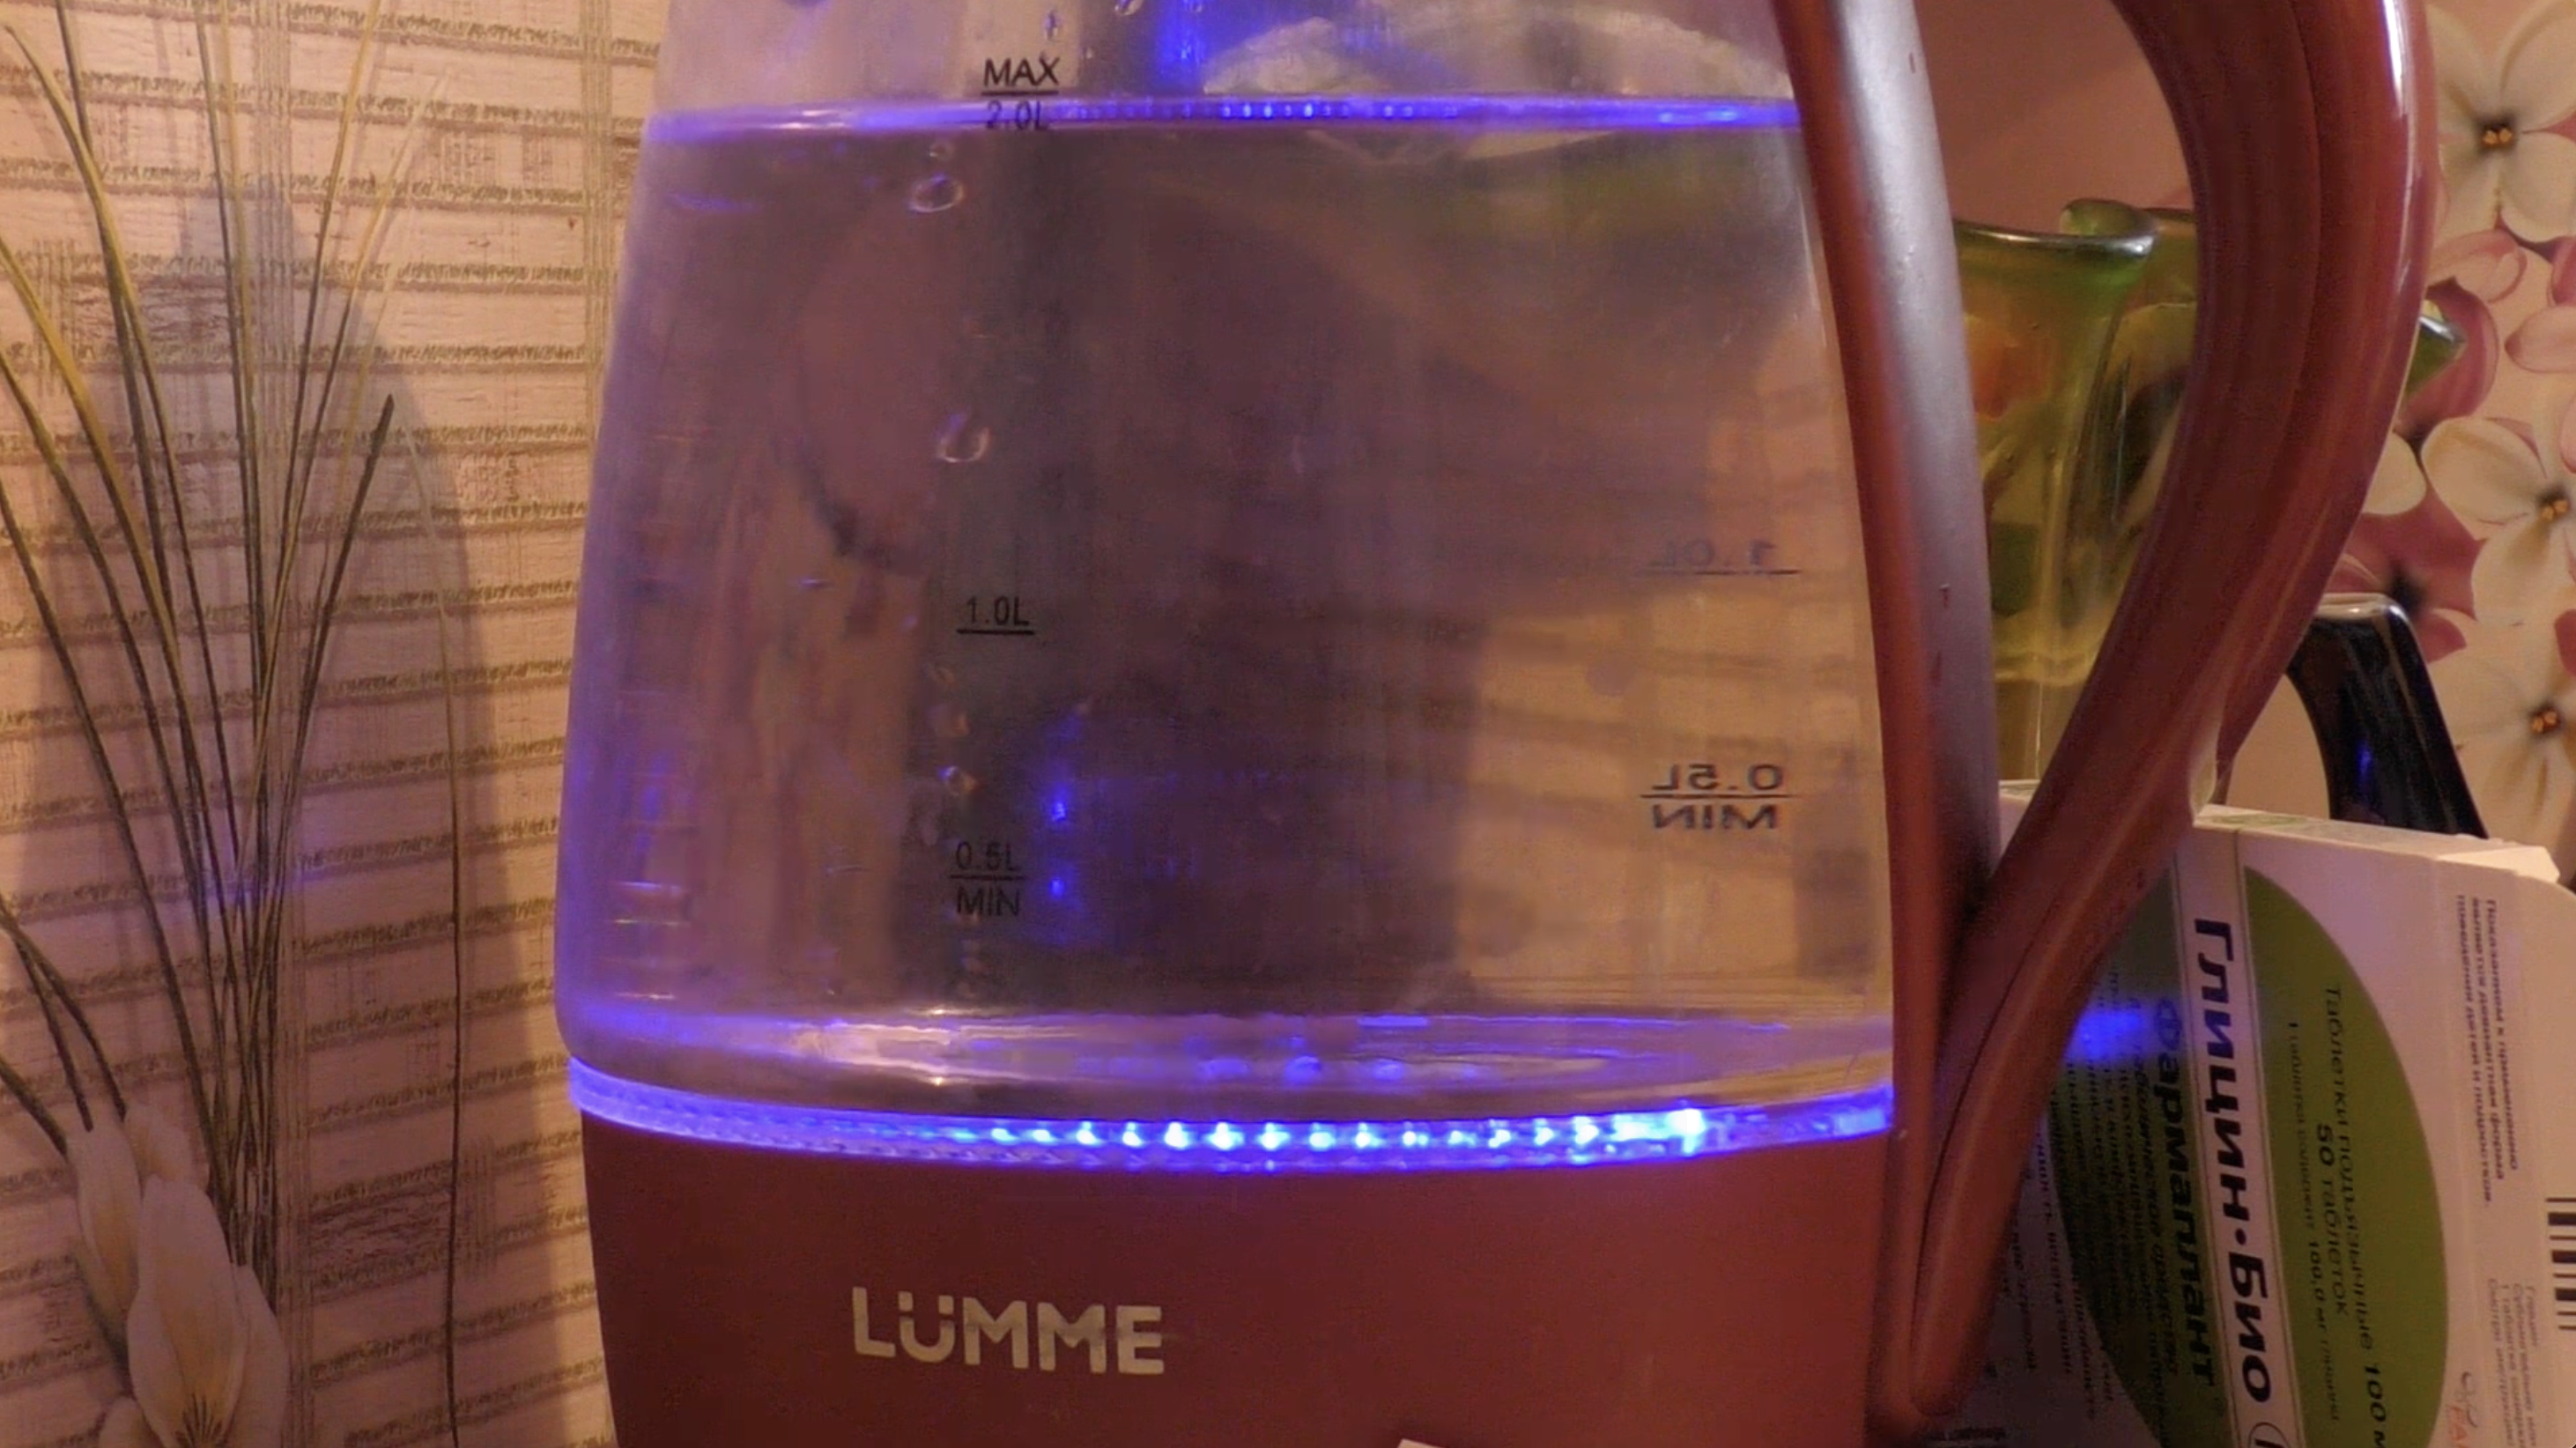
\includegraphics[width=0.8\textwidth]{images/image.png}
	\caption{Графический результат}
	\label{fig:syntdiag}
\end{figure}

\newpage
\section*{Заключение}
\addcontentsline{toc}{section}{Заключение}
В ходе выполнения лабораторных работ были изучены некоторые аспекты автоматизации тестирования программного обеспечения. Основное внимание было уделено созданию и написанию юнит-тестов с использованием JUnit, организации и выполнению тестов с помощью Selenium WebDriver и TestNG. Эти навыки и инструменты повышают эффективность и качество процесса тестирования программного обеспечения.
\newpage
\section*{Список источников}
\addcontentsline{toc}{section}{Список источников}
\begin{enumerate}
	\item Курс лекций по атоматизированному тестированию. Спасов Г.Е.
\end{enumerate}
\end{document}